\documentclass{article}
\usepackage[utf8]{inputenc}
\usepackage{graphicx}
\usepackage[many]{tcolorbox}
\usepackage{setspace}
\usepackage{multicol}
\usepackage{hyperref}
\usepackage[margin=1in]{geometry}

\hypersetup{
    colorlinks=true,
    linkcolor=blue,
    filecolor=magenta,
    urlcolor=cyan,
    citecolor=cyan
}

\definecolor{main}{HTML}{5989cf}
\definecolor{sub}{HTML}{cde4ff}


\newtcolorbox{boxH}{
    colback = sub,
    colframe = main,
    boxrule = 0pt,
    leftrule = 6pt
}

\urlstyle{same}

\begin{document}

\title{COVID-19 Victims Database Project}
\author{Livxy}
\date{March 2023}

\maketitle
\thispagestyle{empty}
\vspace{50cm}
\setlength{\columnsep}{14pt}


\section{Introduction}
\begin{boxH}
	This project is still in progress, and the data is only from the United States. (Not including Alaska, Hawaii, and Puerto Rico for visualization purposes.)
\end{boxH}

\indent

The COVID-19 pandemic has caused a lot of deaths and has affected many people.\
The goal of this project is to collect and analyze data related to COVID-19 victims and to gain insights into the survivability of having COVID-19 and contacting it.\
The project can also help us identify high-risk groups and take measures to protect them.


\section{Data Collection}
\indent

The data collection process is automated using Python.\
The data is collected from the following sources: \
\begin{itemize}
	\item \cite{census} \url{https://hifld-geoplatform.opendata.arcgis.com/datasets/us-county-boundaries} - US county boundaries from the US Census Bureau
	\item \cite{cutrer} \url{https://github.com/joncutrer/geopandas-tutorial/tree/master/data} - Map data from Jon Cutrer
	\item \cite{nytimes} \url{https://github.com/nytimes/covid-19-data} - COVID-19 live data from the New York Times
\end{itemize}



\section{Survivability Analysis}


\section{Visualization}

% \begin{figure}[h]
%     \centering
%     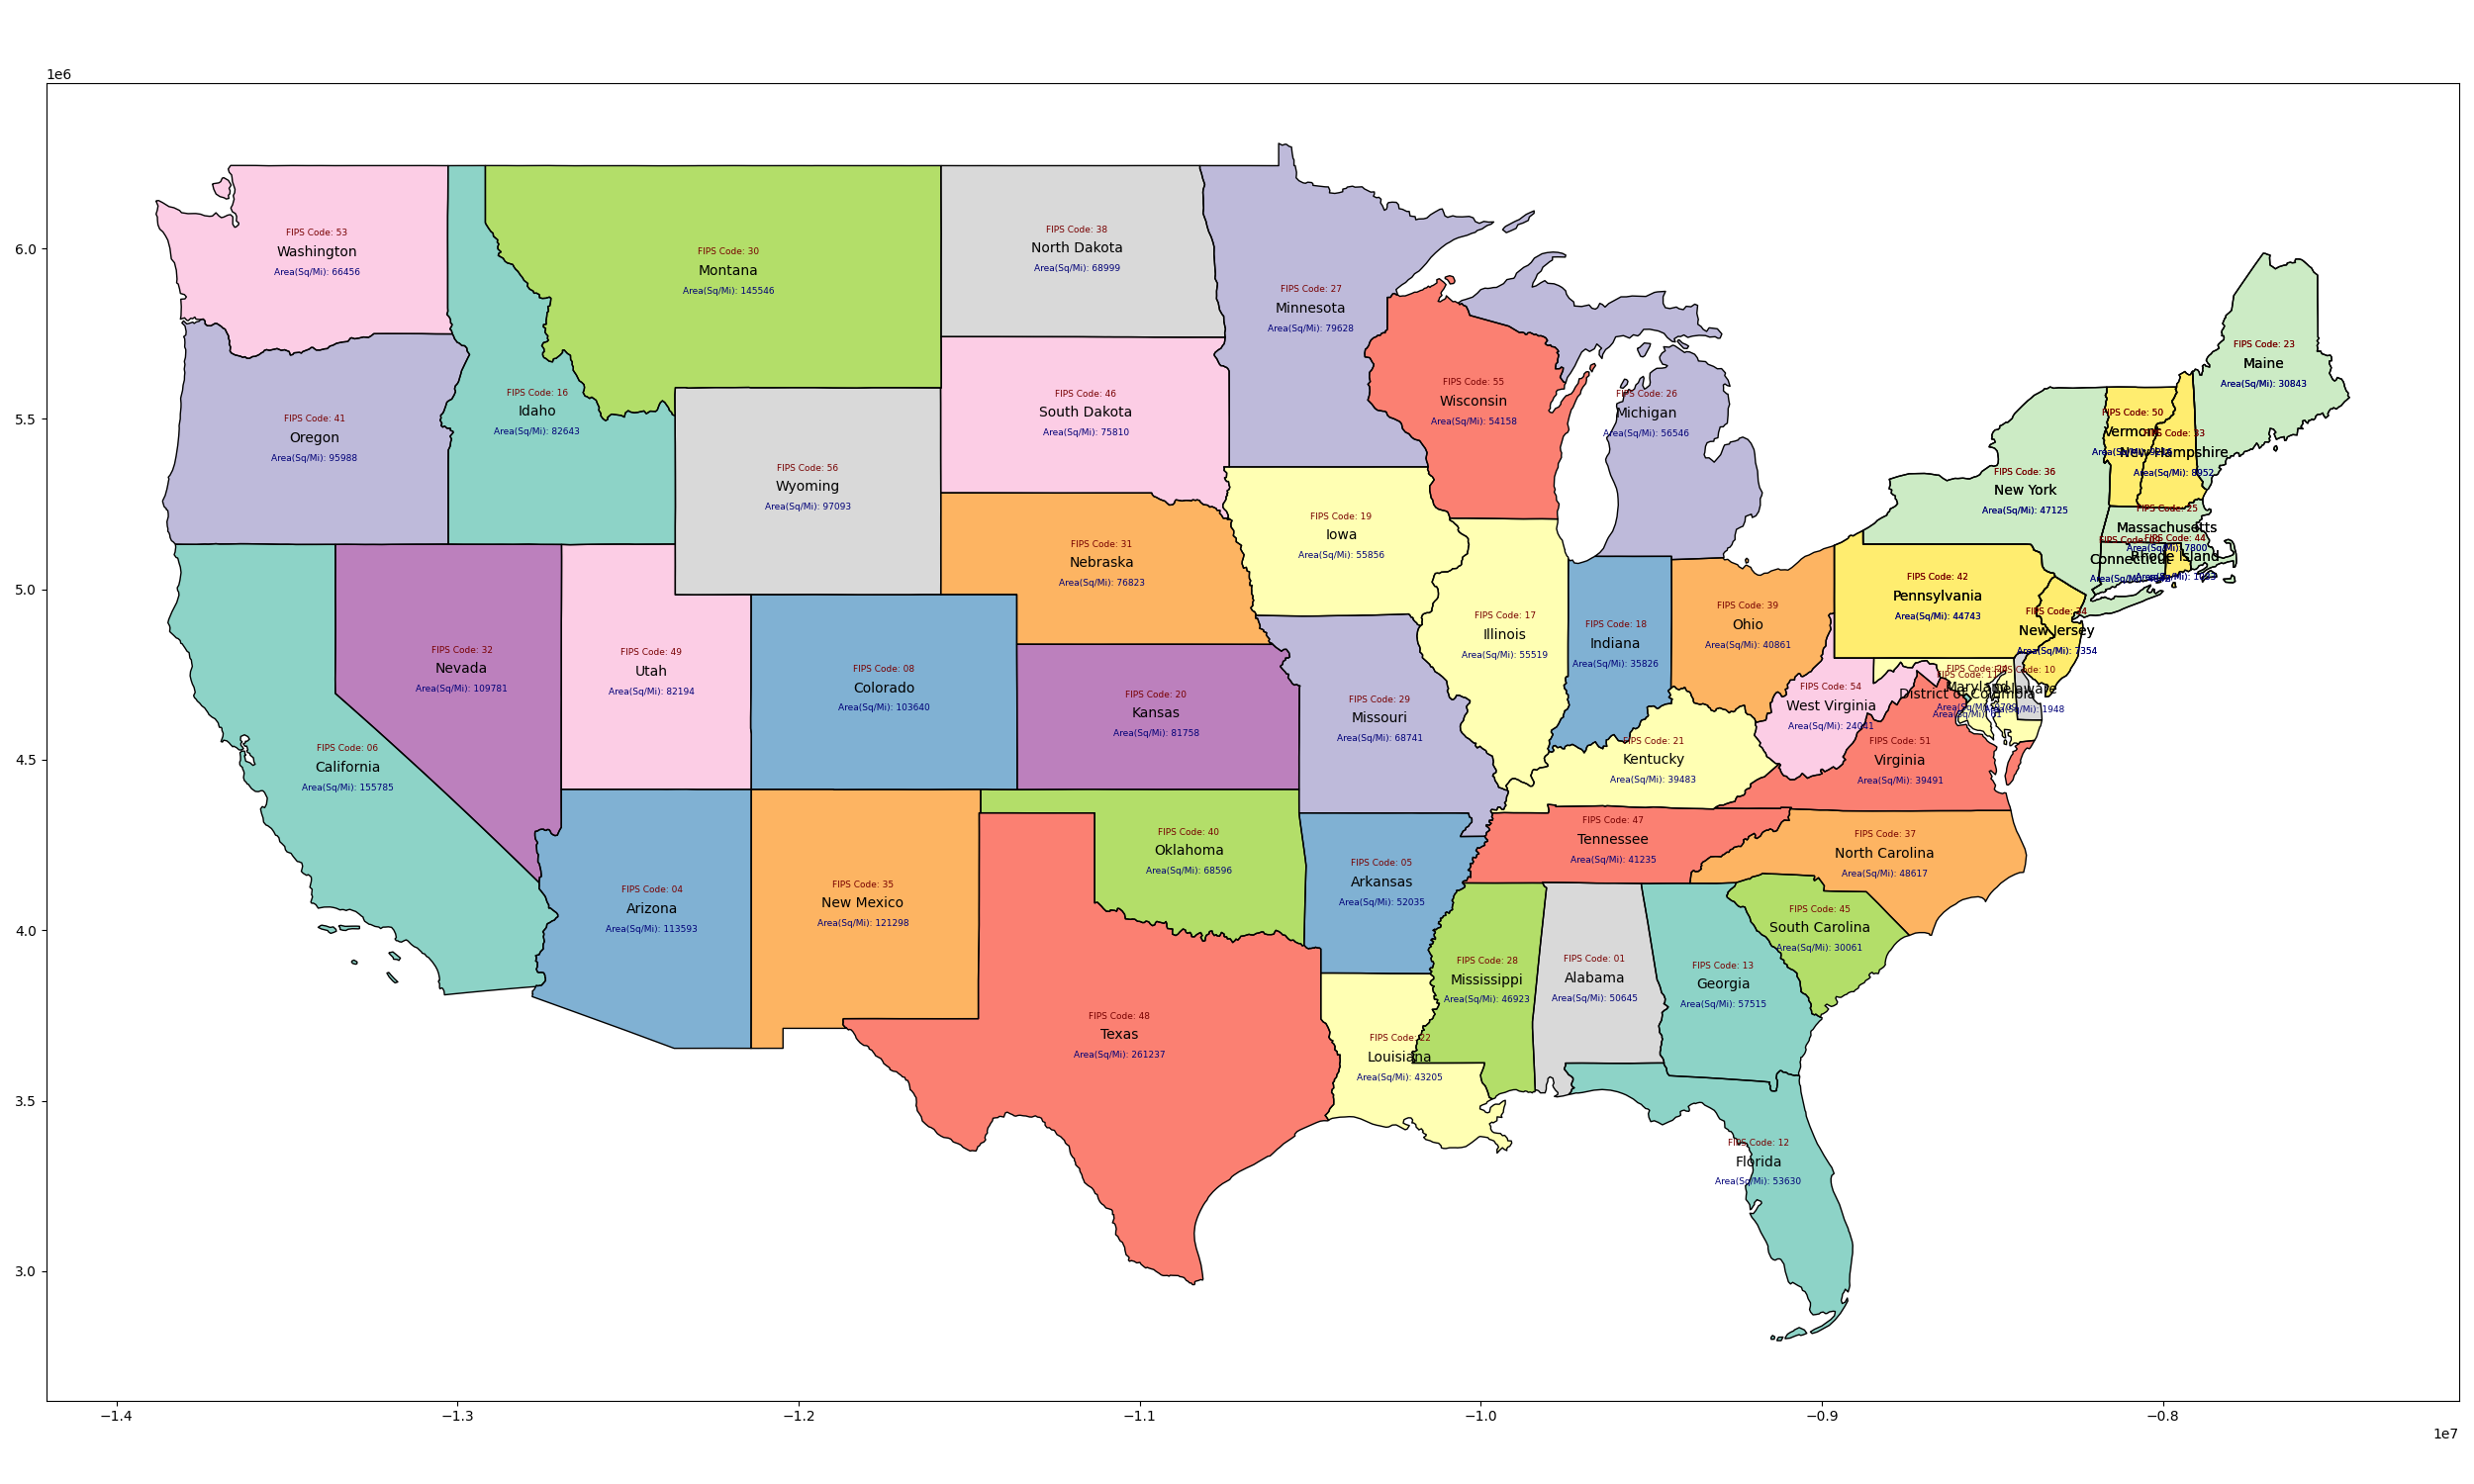
\includegraphics[width=1\textwidth]{images/USA.png}
%     % \caption{COVID-19 victims in the US}
% \end{figure}

\section{Conclusion}

\indent

By collecting and analyzing data related to COVID-19 victims, we can gain insights into the survivability of having COVID-19 and contacting it.\
The project can also help us identify high-risk groups and take measures to protect them.\
By using Python to automate the data collection and analysis process, we can save time and resources and focus on the analysis and interpretation of the data.

\section{Credit}

\bibliographystyle{plain}
\bibliography{extra/paper}

\end{document}